\chapter{Método Proposto}      \label{Metodo Proposto}

No Capítulo anterior, foram discutidos os conceitos básicos da \textit{nanofotônica} e do \textit{aprendizado de máquina}. Neste Capítulo, será abordado o procedimento de otimização e modelagem inversa por \textit{aprendizagem profunda} dos dispositivos fotônicos estudados neste trabalho, desde a geração do banco de dados à escolha da arquitetura de rede neural. Na na Seção \ref{Aplicacao Circulador}, o leitor encontrará a metodologia de modelagem inversa aplicada aos dois circuladores baseados em cristais fotônicos.


\section{Descrição do Problema}

Em sistemas de comunicações, os dispositivos nanofotônicos desempenham um papel importante enquanto componentes não-recíprocos, como isoladores, chaves, circuladores e divisores de potência (alguns desses dispositivos são discutidos em \cite{dmitriev2012nonreciprocal,dmitriev2014magneto,dmitriev2019dynamically,dmitriev2013optical}). Uma das tarefas fundamentais nas quais esses dispositivos desempenham em circuitos integrados é na proteção de fontes eletromagnéticas contra possíveis reflexões do sinal de diferentes partes do circuito ocasionando, desta forma, na transmissão deste sinal para apenas partes desejadas do circuito \cite{hines1971reciprocal}.

\begin{figure}[H]
    \centering
    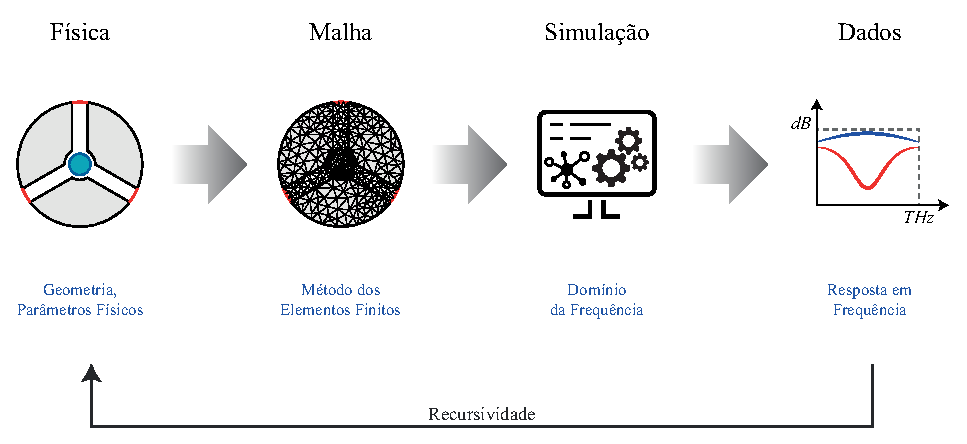
\includegraphics{04-Figuras/DirectModeling.eps}
    \caption{Modelagem convencional no COMSOL Multiphysics \textregistered.} \par
    Fonte: do Autor.
    \label{fig: DirectModeling}
\end{figure}

Esses dispositivos podem ser estudados e construídos a partir de simulações computacionais, por exemplo, por intermédio do software COMSOL Multiphysics \textregistered, em etapas conforme mostradas na Fig. \ref{fig: DirectModeling}. Nesse sentido, esse estudo perpassa pelas seguintes etapas:

\begin{itemize}
    \item Física: avaliação da geometria e parâmetros físicos de operação do dispositivo;
    \item Malha: processo de discretização do dispositivo através do Método dos Elemento Finitos;
    \item Simulação: início da simulação computacional no domínio da frequência.
    \item Dados: após finalizada a simulação, são gerados dados, como a resposta em frequência do dispositivo.
\end{itemize}

Modelar esses dispositivos através de simulação computacional é uma tarefa que pode envolver um alto custo computacional conforme aumenta a complexidade desses dispositivos \cite{noureen2021deep,valkanas2019neural}. Em métodos tradicionais de modelagem, cabe ao projetista a recursividade para conferir manual e empiricamente as relações de geometria do dispositivo para com a resposta em frequência. Deve-se repetir esse procedimento tantas vezes quanto forem necessárias a fim de garantir uma resposta em frequência considerada ótima (deve-se avaliar enquanto parâmetro de qualidade, por exemplo, se as curvas de transmissão e isolamento estão em ressonância na frequência central de operação do dispositivo, bem como a sua largura de banda).

Por outro lado, à medida que a inteligência artificial evoluiu significativamente nas últimas décadas no campo da \textit{aprendizagem profunda}, uma nova abordagem de modelagem de geometria de dispositivos emergiu nos últimos, como mostra a Fig. \ref{fig: InverseDesign}.

\begin{figure}[H]
    \centering
    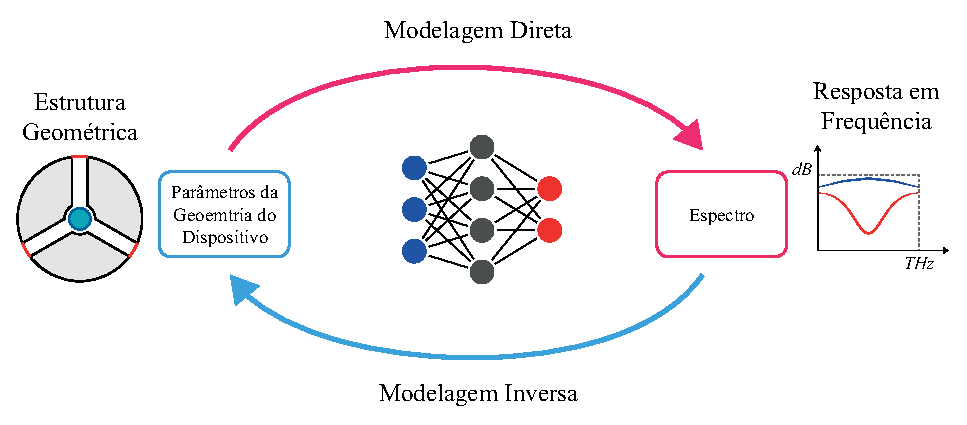
\includegraphics{04-Figuras/InverseDesign.eps}
    \caption{Esquemático dos tipos de modelagens.} \par
    Fonte: do Autor.
    \label{fig: InverseDesign}
\end{figure}

A proposta é realizar a modelagem do dispositivo a partir da sua resposta em frequência, dada uma condição de operação considerada ótima ou ideal. Nesse estudo, uma rede neural profunda é usada para mapear as variadas combinações de geometria com as respectivas respostas em frequência do dispositivo para, então, extrair um modelo de aprendizagem.


\section{Otimização por Aprendizado Profundo}

Nessa abordagem, uma rede neural profunda pode aprender como a geometria do dispositivo está relacionada com sua própria resposta em frequência. Esse processo de otimização é conhecido como \textit{modelagem inversa} da geometria \cite{liu2018training,malkiel2017deep,peurifoy2018nanophotonic}, já que é um procedimento contrário ao convencional, isto é, enquanto que na modelagem convencional contrói-se primeramente a geometria do dispositivo para se obter a resposta em frequência a partir do seu funcionamento, neste procedimento proposto de otimização e modelagem inversa por rede neural profunda, partiremos de uma resposta em frequência ideal a qual será apresentada à rede neural já treinada, que retornará a geometria que está associada a esta resposta em frequência ideal. Resumidamente, dada uma resposta em frequência ideal (desejada), a rede neural irá modelar a geometria do dispositivo para que esse objetivo seja atingido.

Todo esse procedimento de otimização envolve as etapas seguintes etapas básicas:

\begin{enumerate}
	\item \textbf{Estudo Inicial:} nesta etapa, são verificadas as características dos dispositivos, como a sua modelagem geométrica e resposta em frequência. Esse estudo é importante para avaliar quais parâmetros devem ser levados em consideração para a otimização do dispositivo.
	\item \textbf{Construção do Banco de Dados:} consiste em montar um banco de dados contendo as características de geometria de dispositivo relacionadas com a respectiva resposta em frequência. Esse procedimento foi realizado usando os softwares COMSOL e o MATLAB.
	\item \textbf{Rede Neural Profunda:} a rede neural foi construída na linguagem de programação Python com o uso do framework TensorFlow. O objetivo desse procedimento é extrair um modelo de aprendizagem para tornar as predições com maior acurácia. No final desse processo, é esperável que a rede neural (\textit{deep learning}) aprenda qual é a geometria mais otimizada para os dispositivos estudados.
	\item \textbf{Algoritmo de Otimização:} todo o procedimento de otimização envolve vários serviços e programas e, a fim de automatizar todo esse processo, foi desenvolvido também um script que concatena todos as etapas usadas para a otimização. O objetivo é esse algoritmo de otimização rodar até que o modelo otimizado seja encontrado.
\end{enumerate}


\subsection{Construção do Banco de Dados}

O procedimento de otimização por inteligência artificial envolve, primeiramente, coletar os dados do problema e organizá-los em um banco de dados. Estes dados foram coletados por meio da API (\textit{Application Programming Interface}, ou ainda em português, Interface de Programação de Aplicativos) que o próprio COMSOL oferece. Uma API permite que aconteça troca de informações entre dois ou mais sistemas. Neste caso, a API \textit{COMSOL LiveLink for MATLAB} \cite{livelink2021matlab} permite que o MATLAB possa controlar como as simulações numéricas do COMSOL acontecem, desde o processo de automatizá-las à triagem desses dados para a construção do banco de dados.

Os dispositivos nanofotônicos são modelados e estudados a partir do software de simulação eletromagnética COMSOL. Nessa etapa, o próprio projetista constrói o dispositivo com as características geométricas e de operação que ele deve ter. Uma vez que esse estudo esteja estabelecido, o próximo passo é mapear variáveis que mais influenciam na resposta em frequência do dispositivo. Assim, cada variável será responsável por realizar uma determinada modificação na geometria do dispositivo. Nesse ponto, deve-se atentar que essas variáveis geométricas devem respeitar a condição de simetria dos dispositivos. Isso é necessário pois é realizado um estudo embasado na \textit{teoria de grupos} \cite{vvedensky2009symmetry}, a qual permite reduzir a quantidade de cálculos da matriz de espalhamento do dispositivo.

As mesmas variáveis que modificam simetricamente a geometria do dispositivo são carregadas em um \textit{script} no MATLAB. A ideia por trás desse script é automatizar as simulações em \textit{Loops}\footnote{Neste trabalho, o termo \textit{Loop} é usado para designar um conjunto de várias simulações.} de execução. Desta maneira, a cada execução do script o MATLAB atribui valores randômicos para essas variáveis. Em termos práticos, isso significa que cada simulação de dispositivo háverá uma geometria diferente para simular. Ao final de cada simulação, os dados randômicos de geometria e a respectiva resposta em frequência são exportados em vários arquivos com a extensão \textit{.txt} e amarzenados em um diretório definido no mesmo script do MATLAB.

Foi desenvolvido, também, um outro script no MATLAB que é resposável por ler os dados gerados pelas simulações automatizadas. A função desse \textit{script} é ler todos os arquivos de simulação que foram gerados e montar o banco de dados em um único arquivo, onde os dados estão organizados de maneira sequencial (conforme o Loop de simulação) e normalizados no intervalo $0\dotso 1$, como mostrado na Fig. \ref{fig: DatasetBuilding}.

\begin{figure}[H]
    \centering
    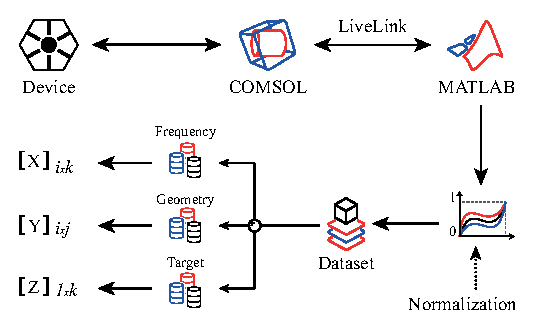
\includegraphics{04-Figuras/DatasetBuilding.eps}
    \caption{Procedimento de contrução do banco de dados.} \par
    Fonte: do Autor.
    \label{fig: DatasetBuilding}
\end{figure}

Assim, nessa etapa, são gerados três arquivos na extensão \textit{.csv}, cada qual entendidos como tensores, a saber:

\begin{itemize}
	\item \textbf{Resposta em Frequência} -- definido pelo tensor $[X]$, compreende as amplitudes discretizadas em 51 pontos de gráfico de cada curva da resposta em frequência, sequenciadas linha-a-linha.
	\item \textbf{Geometria} -- definido pelo tensor $[Y]$, compreende o agrupamento de cada valor randômico de parâmetros de geometria.
	\item \textbf{Espectro Desejado} -- definido pelo tensor $[Z]$, compreende à resposta em frequência desejada para o dispositivo (construída manualmente no MATLAB).
\end{itemize}

Esses arquivos podem ser visualizados na forma de tensores que alimentarão a rede neural profunda. A Eq. \ref{eq: tensorY} mostra o tensor $\mathbf{[Y]}$ referente aos dados de geometria do dispositivo.

\begin{equation}
\label{eq: tensorY}
\mathbf{[Y]_{i,j}} =
\begin{bmatrix}
y_{1_{[1,1]}} & y_{2_{[1,2]}} & \cdots & y_{j_{[1,j]}}\\
y_{1_{[2,1]}} & y_{2_{[2,2]}} & \cdots & y_{j_{[2,j]}}\\
\vdots  & \vdots  & \ddots & \vdots\\
y_{1_{[i,1]}} & y_{2_{[i,2]}} & \cdots & y_{j_{[i,j]}}
\end{bmatrix},
\end{equation}

\noindent
onde $j$ é o número total de variáveis que modificam a geometria do dispositivo e $i$ é referente ao número de instâncias, isto é, ao número de simulações totais. O mesmo raciocínio se aplica para a construção do banco de dados da resposta em frequência, a qual é agrupada em um tensor como mostrado na Eq. \ref{eq: tensorX}:

\begin{equation}
\label{eq: tensorX}
\mathbf{[X]_{i,k}} =
\begin{bmatrix}
x_{1_{[1,1]}} & x_{2_{[1,2]}} & \cdots & x_{k_{[1,k]}}\\
x_{1_{[2,1]}} & x_{2_{[2,2]}} & \cdots & x_{k_{[1,k]}}\\
\vdots  & \vdots  & \ddots & \vdots\\
x_{1_{[i,1]}} & x_{2_{[i,2]}} & \cdots & x_{k_{[i,k]}}
\end{bmatrix}.
\end{equation}

Note que o número de instâncias $i$ precisa ter o mesmo tamanho para $\mathbf{[X]}$ e $\mathbf{[Y]}$, uma vez que geometria e resposta em frequência estão relacionadas. Por fim, o \textit{espectro desejado}\footnote{O termo \textit{espectro desejado} tem o mesmo significado de \textit{resposta em frequência desejada}.} é definido como um tensor, assim mostrado na Eq. \ref{eq: tensorZ}.

\begin{equation}
\label{eq: tensorZ}
\mathbf{[Z]_{1,k}} =
\begin{bmatrix}
z_{1_{[1,1]}} & z_{2_{[1,2]}} & \cdots & z_{k_{[1,k]}}\\
\end{bmatrix}.
\end{equation}

Como já mencionado, o tensor $\mathbf{[Z]}$ foi feito considerando as características ideais de operação do dispositivo em sua resposta em frequência. É importante ressaltar que a dimensão $k$ dos tensores $\mathbf{[X]}$ e $\mathbf{[Z]}$ tem o mesmo tamanho (número de colunas). Nesse sentido, $k$ é definido dado o número de curvas da resposta em frequência (parâmetro que depende de cada dispositivo avaliado) e o quão essas curvas estão discretizadas (previamente comentado, em 51 pontos). Essa análise está melhor elucidada na Seção \ref{Aplicacao Circulador} deste Capítulo.

Todo o banco de dados é normalizado no intervalo $0\dotso 1$, conforme a Eqs. \ref{eq: normalizacaoY}, \ref{eq: normalizacaoX} e \ref{eq: normalizacaoZ}:

\begin{equation}
\label{eq: normalizacaoY}
N_{[Y]} = \frac{DataSet[Y] - MinDataSet[Y]}{MaxDataSet[Y] - MinDataSet[Y]},
\end{equation}

\begin{equation}
    \label{eq: normalizacaoX}
    N_{[X]} = \frac{DataSet[X] - MinDataSet[X]}{MaxDataSet[X] - MinDataSet[X]},
\end{equation}

\begin{equation}
    \label{eq: normalizacaoZ}
    N_{[Z]} = \frac{DataSet[Z] - MinDataSet[Y]}{MaxDataSet[Y] - MinDataSet[Y]},
\end{equation}

\noindent
onde $N_{[Y]}$, $N_{[X]}$ e $N_{[Z]}$ são as respectivas normalizações dos tensores $\mathbf{[Y]}$, $\mathbf{[X]}$ e $\mathbf{[Z]}$. Esse procedimento é necessário, pois a rede neural irá usar um método recursivo para minimizar uma \textit{função custo} usando a descida do \textit{gradiente descedente} \cite{bottou2010large,geron2019hands} e, desta forma, reduzir a influência de valores grandes no banco de dados em relação aos valores pequenos, de forma a redimensionar o banco de dados sem distorcer as diferenças nos intervalos entre cada valor. Dados muito dispersos (portanto, alto desvio padrão) podem tornar o algoritmo de otimização da rede neural mais lento, ou até mesmo provocar a não-convergência da descida do gradiente \cite{geron2019hands}.


\subsection{Rede Neural Profunda}

A rede neural tem por objetivo extrair um modelo de aprendizagem a partir do banco de dados previamente montado, como ilustrado na Fig. \ref{fig: StepNetwork-a}.

\begin{figure}[H]
    \centering
    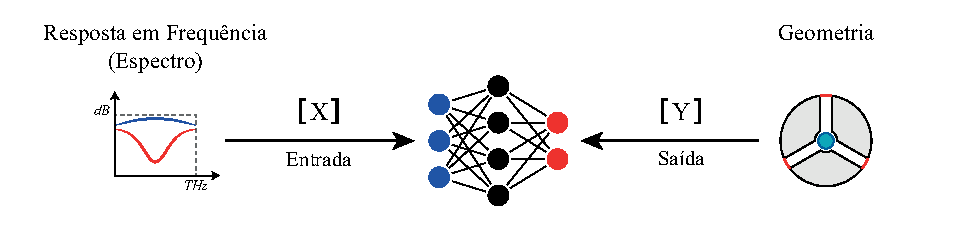
\includegraphics{04-Figuras/StepNetwork-a.eps}
    \caption{Esquema básico da alimentação do banco de dados na rede neural.} \par
    Fonte: do Autor.
    \label{fig: StepNetwork-a}
\end{figure}

Para a construção da rede neural profunda foi utilizada a biblioteca de código aberto para Aprendizado de Máquina \textit{Tensorflow} \cite{tensorflow2015whitepaper} no ambiente da linguagem de programação Python \cite{van1995python}.

\begin{figure}[H]
    \centering
    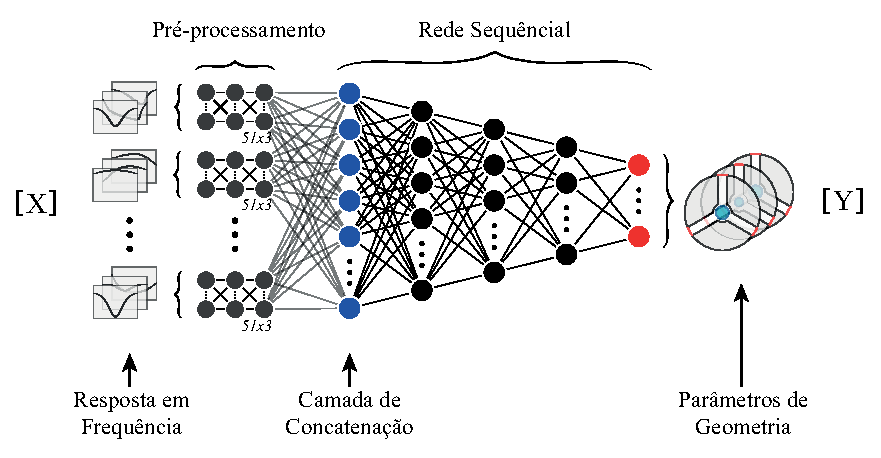
\includegraphics{04-Figuras/StepNetwork-b.eps}
    \caption{Arquitetura da rede neural profunda detalhada.} \par
    Fonte: do Autor.
    \label{fig: StepNetwork-b}
\end{figure}

A Fig. \ref{fig: StepNetwork-b} mostra a arquitetura detalhada da rede neural e o esquemático de como o banco de dados é alimentado através dela. O tensor $[X]$ é alimentado através da entrada da rede, passando por uma camada de \textit{pré-processamento paralelo}, desta forma, cada estrutura em paralelo cuidará de fazer um pré-processamento de cada curva individualmente. Posteriormente, os dados seguem para uma camada de concatenação e, então, propagados adiante através da \textit{rede sequencial} onde, na saída de toda a rede, estará o tensor de parâmetros de geometria $[Y]$.

A rede neural, primeiramente, passa pelo processo de treinamento, onde ela aprenderá iterativamente a modelagem das relações da geometria do dispositivo com a sua resposta em frequência. Posteriormente, a rede neural passará pelo processo de predição, isto é, após ela ter extraído um modelo de aprendizagem do dispositivo, agora irá predizer qual geometria deve-se ter, dada uma resposta em frequência ideal.


\subsection{Treinamento e Predição}

No processo de treinamento da rede neural profunda, foi utilizado o algoritmo de aprendizagem \textit{Adam} e, como função custo, o erro médio quadrático (do inglês, \textit{mean squared error} (MSE)). O processo de treinamento é feito minimizando a função custo, $C$, mostrada na Eq. \ref{eq: costFunction}.

\begin{equation}
\label{eq: costFunction}
C = \frac{1}{n}\sum_{i=1}^{n}\left ( Y_{i} - \hat{Y}_{i} \right )^{2}.
\end{equation}

A partir das métricas do MSE, pode-se estimar a performance da rede neural profunda. Na Eq. \ref{eq: costFunction}, o parâmetro $i$ é o mesmo \textit{número de instâncias} anteriormente mencionado, $n$ é o número de execuções de simulações (\textit{Loop}) e os argumentos $Y_{i}$ e $\hat{Y}_{i}$ são os vetores de \textit{geometria real} e \textit{geometria prevista}, respectivamente. Nesse aspecto, a função custo $C$ mede o erro entre a \textit{geometria real} $Y_{i}$ e \textit{geometria prevista} $\hat{Y}_{i}$. Desse modo, o caso ideal é quando a função custo $C$ for o mais próxima quanto possível de zero. Em termos práticos, isso indica que não há mais erro sgnificativo entre a predição e o valor real da geometria e, assim, a rede neural se tornou apta a predizer qual é a geometria que está relacionada à resposta em frequência desejada.

Após o processo de treinamento, a rede neural poderá fazer a predição da geometria dada um espectro desejado. Os dados da saída da rede contém um vetor (ainda normalizado) com as variáveis de geometria que deverão, posteriormente, ser simuladas no COMSOL para a validação da predição da rede neural. É necessário \textit{desnormalizar} esse vetor para a devida simulação.

\begin{equation}
    \label{eq: desnormalizacaoW}
    D_{[Y]} = Net[W] \times \left ( MaxDataSet[Y] - MinDataSet[Y] \right ) + MinDataSet[Y]
\end{equation}

Na Eq. \ref{eq: desnormalizacaoW}, $Net[W]$ refere-se ao vetor de saída da rede na etapa de predição (ainda normalizado), e $D_{[Y]}$ é o vetor de geometria desnormalizado. Nesse processo, a desnormalzação será feita usando os mesmo valores de máximo e mínimo da Eq. \ref{eq: normalizacaoY}.

O banco de dados foi dividido em $80\%$ para dados de \textit{treinamento}, $10\%$ para \textit{validação} e $10\%$ para \textit{teste}. Em termos práticos, isso significa que a rede neural terá apenas $80\%$ para treinar as amostras de geometria e resposta em frequência. Posteriormente, durante a fase de teste, a rede neural será submetida a $10\%$ do banco de dados, sobre o qual ela não teve conhecimento prévio (ou seja, não foi enviesada pela amostra). E é neste momento que o poder de predição será avaliado.


\subsection{Procedimento de Otimização}

Muitos serviços são executados em etapas, desde o momento em que o banco de dados é extraído e montado, ao momento de validação da predição da rede neural. Assim, foi desenvolvido um script que automatiza a comunicação entre esses serviços (COMSOL, MATLAB e PYTHON/TENSORFLOW).

Todos eles são integrados dinamicamente por meio de um algoritmo executado a partir do terminal do computador. Assim, como ilustrado na Fig. \ref{fig: OptimizationAlgorithm}, o algoritmo pode ser executado automaticamente quantas vezes forem necessárias (até que a otimização seja concluída, por exemplo).

\begin{figure}[H]
    \centering
    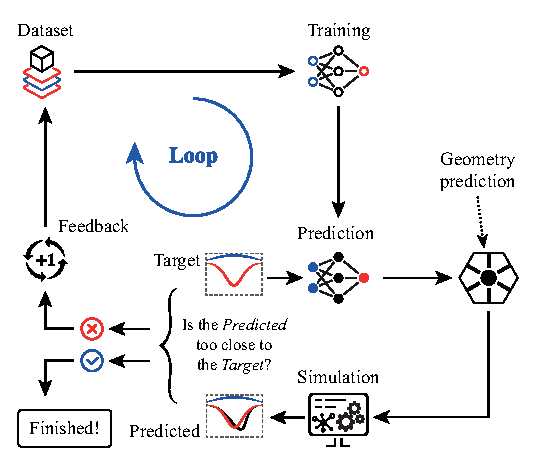
\includegraphics{04-Figuras/OptimizationAlgorithm.eps}
    \caption{Algoritmo de otimização.} \par
    Fonte: do Autor.
    \label{fig: OptimizationAlgorithm}
\end{figure}

Como ponto de partida, foi gerado um \textit{Loop} de 100 simulações aleatórias, contendo as mais diversas variações de geometria e respectiva resposta em frequência, a fim de construir um banco de dados inicial, denotado por $i_{0}$ na Fig. \ref{fig: loopAlgorithm}.

%\begin{equation}
%    \label{eq: StartLoop}
%    i_{0} = \sum_{i=1}^{100}\left ( i \right ).
%\end{equation}

Esse número inicial (100 instâncias iniciais no banco de dados) é necessário para se averiguar a melhor arquitetura de rede que se adapta a cada problema. Nesse ponto, várias arquiteturas de redes neurais com diferentes configurações de neurônios e camadas intermediárias serão avaliadas através das métricas de desempenho do erro médio quadrático com a finalidade de se trabalhar com a melhor rede neural. Superando essa necessidade da arquitetura de rede, os \textit{Loops} de simulações continuam a partir de $i_{0}$, como mostrado na Fig. \ref{fig: loopAlgorithm}.

%\begin{equation}
%    \label{eq: Loop}
%    Loop = i_{0} + \sum_{i=i_{0}+1}^{n}\left ( i \right ).
%\end{equation}


\begin{figure}[H]
    \centering
    \includegraphics{04-Figuras/loopAlgorithm.eps}
    \caption{Diagrama de blocos simplificado do algoritmo de otimização.} \par
    Fonte: do Autor.
    \label{fig: loopAlgorithm}
\end{figure}


Vale ressaltar que cada dispositivo submetido ao procedimento de modelagem inversa tem o seu próprio banco de dados e, portanto, o procedimento de otimização funciona de forma totalmente independente para cada um.

Seguindo com o algoritmo, a rede neural profunda será treinada com o banco de dados por $20000$ épocas. Posteriormente, na fase de \textit{predição}, será apresentado o tensor $[Z]$ contendo o espectro desejado. A rede neural, então, retorna os parâmetros de geometria que serão desnormalizados (ver Eq. \ref{eq: desnormalizacaoW}) e, posteriormente, simulados no COMSOL via \textit{API LiveLink for MATLAB}. A resposta em frequência resultante da simulação é então comparada com o \textit{espectro desejado}. Nesse momento, o algoritmo toma uma decisão: se a resposta em frequência \textit{prevista} (simulada) está satisfatoriamente próximo ao \textit{desejado}, o procedimento de otimização é finalizado. Isso significa que a geometria do dispositivo com a resposta de frequência contendo parâmetros ótimos de operação foi encontrada. Porém, se o resultado da simulação não for satisfatório, esse resultado não é descartado, mas sim realimentado no banco de dados na fase de \textit{feedback}. Como consequência, isso incrementa mais uma instância ($i + 1$) no banco de dados. Dessa forma, da próxima vez que o algoritmo for executado, a rede neural saberá que essa ainda não é a solução.


\section{Fatores de Qualidade}

Foram realizadas algumas avaliações de fatores que aferem a qualidade dos dispositivos estudados. Este estudo é necessário para se averiguar as possiveis melhoras em termos de desempenho dos dispositivos proporcionados pelo método de otimização por aprendizado de máquina. Esses \textit{fatores de qualidade} são características da resposta em frequência inerente a cada dispositivo estão descritos como se segue:

\begin{itemize}
	\item \textbf{Frequência central}: todas as curvas dos parâmetros-S ($S_{ij}$) são avaliadas quanto à ressonância na frequência central de operação do dispositivo. Esse fator é avaliado por $\Delta F_{ij}$, que afere a distância do ponto de inflexão da curva avaliada à $F_{c}$ (frequência central). Um fator ótimo ou ideal é quando $\Delta F_{ij} = F_{c}$.
	\item \textbf{Transmissão}: as curvas relacionadas à transmissão são avaliadas quanto à proximidade de -1 dB. Esse fator é avaliado por $\Delta T1_{ij}$. Um valor considerado ótimo é quando $\Delta T1_{ij} = \textrm{-1 dB}$.
	\item \textbf{Isolamento e reflexão}: as curvas relacionadas ao \textit{isolamento} e \textit{relfexão} são avaliadas quanto à proximidade do limiar de -20 dB. Esse fator é avaliado por $\Delta T2_{ij}$. Um valor considerado ótimo é quando $\Delta T2_{ij} \leq \textrm{-20 dB}$.
	\item \textbf{Largura de banda}: a largura de banda do dispositivo é avaliada a -15 dB. Esse fator é avaliado por $BW = f_{2} - f_{1}$, onde $f_{1}$ e $f_{2}$ são referentes às curvas mais internas (mais próximas à $F_{c}$). Um valor considerado ótimo é quando $BW \gg 0$.
\end{itemize}

A Fig. \ref{fig: QualityFactor} ilustra como esses fatores estão relacionados na resposta em frequência.

\begin{figure}[H]
	\centering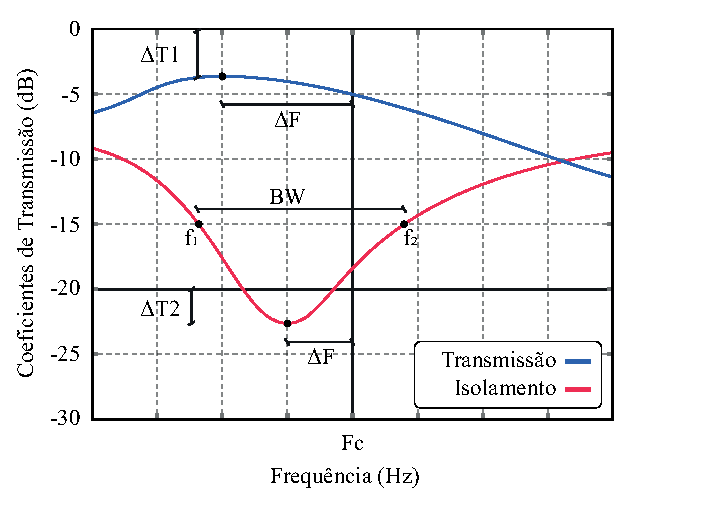
\includegraphics{04-Figuras/QualityFactor.eps}
	\caption{Fatores de qualidade avaliados na resposta em frequência.}
    Fonte: do Autor.
	\label{fig: QualityFactor}
\end{figure}



\section{Aplicação em Circulador}      \label{Aplicacao Circulador}

Os circuldores de junção-T baseados em cristal fotônicos, sendo um com modo de ressonância \textit{dipolo} e outro com modo de ressonância \textit{quadrupolo} discutidos em \cite{DMITRIEV2021100954}, foram submetidos ao procedimento de otimização e modelagem inversa proposto neste trabalho, e apresentam a geometria base indicada na Fig. \ref{fig: PhC_Geometry}.

\begin{figure}[H]
    \centering
    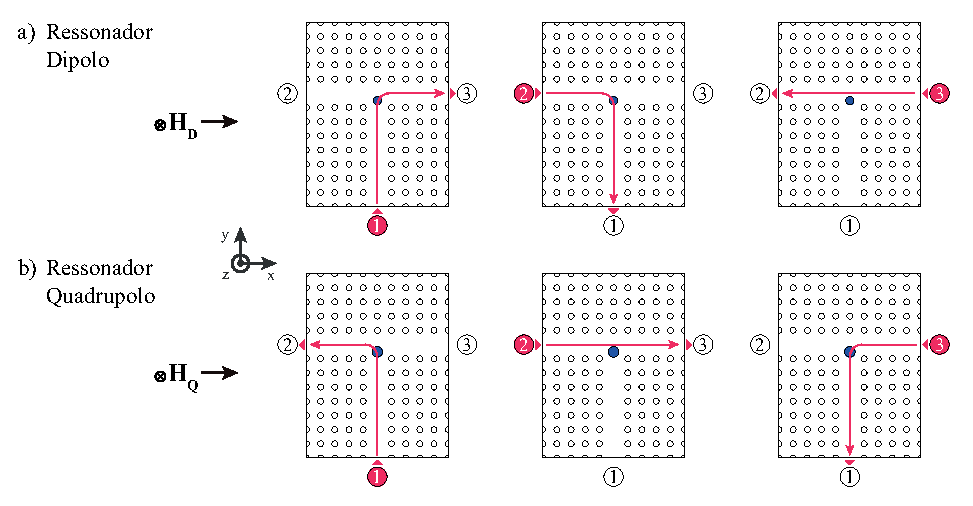
\includegraphics{04-Figuras/PhC_Geometry.eps}
    \caption{Funcionamento dos circuladores. a) Modo dipolo. b) Modo quadrupolo} \par
    Fonte: do Autor.
    \label{fig: PhC_Geometry}
\end{figure}

A resposta em frequência é obtida considerando o desempenho do sinal da \textit{porta 1} para todas as outras e vice-versa. Portanto, $9$ curvas são avaliadas:

\begin{itemize}
    \item Porta 1: $S_{11}$, $S_{21}$, $S_{31}$
    \item Porta 2: $S_{12}$, $S_{22}$, $S_{32}$
    \item Porta 3: $S_{13}$, $S_{23}$, $S_{33}$
\end{itemize}

Conforme a Fig. \ref{fig: PhC_Geometry}, para o circulador \textit{dipolo}, as curvas $S_{31}$, $S_{12}$ e $S_{23}$ devem ser maximizadas (sinal propagado) e as curvas $S_{11}$, $S_{21}$, $S_{22}$, $S_{32}$, $S_{13}$ e $S_{33}$ minimizadas (sinal isolado). A mesma análise se extende para o circulador \textit{quadrupolo}, onde as curvas $S_{21}$, $S_{32}$ e $S_{13}$ devem ser maximizadas (sinal propagado) e as curvas $S_{11}$, $S_{31}$, $S_{12}$, $S_{22}$, $S_{23}$ e $S_{33}$ minimizadas (sinal isolado).

A parametrização da geometria de ambos circuladores foi realizada considerando uma área que, quando modificadas, implicam nas maiores contribuições para o comportamento da resposta em frequência de cada dispositivo. Essa \textit{área de modelagem} está mostrada na Fig. \ref{fig: PhotonicCrystal} e indica a área central da \textit{junção-T}.

\begin{figure}[H]
    \centering
    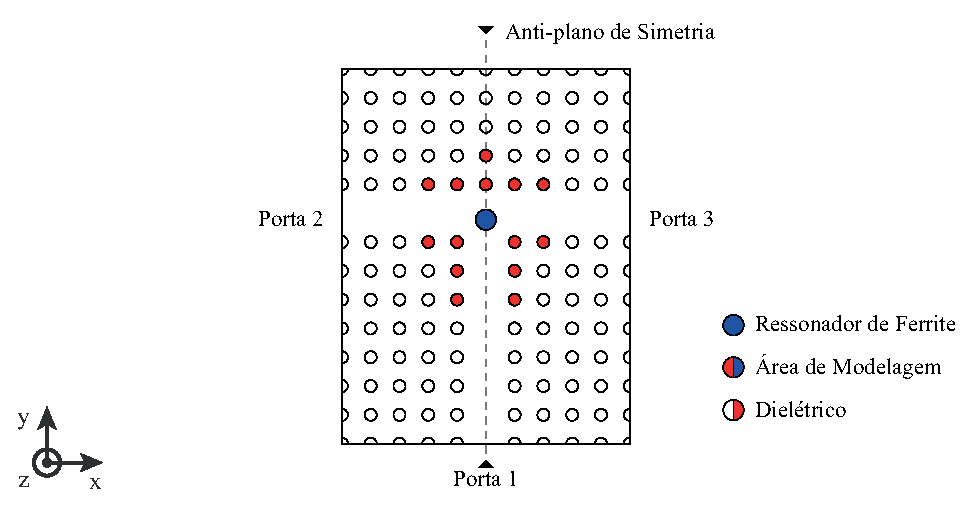
\includegraphics{04-Figuras/PhotonicCrystal.eps}
    \caption{Geometria do cristal fotônico.} \par
    Fonte: do Autor.
    \label{fig: PhotonicCrystal}
\end{figure}

Essas variáveis de geometria incluem os deslocamentos no \textit{eixo-x}, \textit{eixo-y} e o \textit{raio} de cada cilindro, respeitando o eixo de simetria do dispositivo. No total, foram $24$ variáveis de geometria para ambos dispositivos, portanto, o tensor $[Y]$ (alimentado na saída da rede) terá dimensão $i \times 24$ para ambos dispositivos.

Cada curva da resposta em frequência de ambos circuladores está discretizada em 51 pontos e, como em cada porta são avaliadas 3 curvas, portanto, $51 \times 3 \times 3 = 459$. Isso indica que os tensores $[X]$ e $[Z]$ terão dimensão $i \times 459$ e $1 \times 459$, respectivamente. Nesse contexto, a rede neural profunda terá $459$ neurônios na camada de entrada e $24$ neurônios na camada de saída para ambos circuladores.


\subsection{Arquitetura de Rede}

A arquitetura da rede foi definida a partir da quantidade de neurônios nas camadas de entrada e saída. Foram desenvolvidas 6 arquiteturas de redes com diversas configurações de neurônios e camadas.

Definida a quantidade de neurônios nas camadas de entrada e saída da rede neural profunda, o próximo passo foi definir as camadas intermediárias (quantidade de camadas e quantidade de neurônios em cada camada). A escolha igual das mesmas quantidades de variáveis de geometria para ambos circuladores foi intencional, pois facilita o uso de uma arquitetura para trabalhar ambos dispositivos. Foram desenvolvidas 6 arquiteturas de redes com diversas configurações de neurônios e camadas, a saber:

\begin{itemize}
    \item Rede 1: $459 - 200 - 24$
    \item Rede 2: $459 - 200 - 100 - 24$
    \item Rede 3: $459 - 300 - 200 - 100 - 24$
    \item Rede 4: $(51) \parallel \times 9 - 459 - 300 - 200 - 100 - 24$
    \item Rede 5: $(51 - 51 - 51) \parallel \times 9 - 459 - 300 - 200 - 100 - 24$
    \item Rede 6: $(51 - 51 - 51 - 51 - 51 - 51) \parallel \times 9 - 459 - 300 - 200 - 100 - 24$
\end{itemize}

As 6 arquiteturas de redes foram avaliadas com o banco de dados inicial $i_{0}$. Primeiramente, foi realizado o teste de performance das três primeiras redes (\textit{rede 1}, \textit{rede 2} e \textit{rede 3}). Foi observado que a \textit{rede 3} obteve o melhor desempenho (isto é, menor erro). Após essa etapa, mais três arquiteturas foram geradas (\textit{rede 4}, \textit{rede 5} e \textit{rede 6}). Essas redes são variações da \textit{rede 3} contendo nove redes de pré-processamento paralelo (uma para cada curva avaliada), variando em $1$, $3$ e $6$ camadas, as quais são conectadas posteriormente à rede sequencial (propriamente dita, a \textit{rede 3}) através da camada de concatenação.





\begin{table}[H]
    \centering
    \caption{Performance de cada arquitetura de rede em relação ao banco de dados inicial $i_{0}$ de cada circulador.}
    \begin{tabular}{ccc}
\hline
Rede & \multicolumn{1}{r}{Circulador Dipolo (MSE)} & \multicolumn{1}{r}{Circulador Quadrupolo (MSE)} \\ \hline
1    & $3,6307e^{-2}$                              & $4,3351e^{-2}$                                  \\
2    & $2,8347e^{-2}$                   	       & $3,7666e^{-2}$                                  \\
3    & $2,6205e^{-2}$                              & $3,5608e^{-2}$                                  \\
4    & $2,5085e^{-2}$                              & $3,3075e^{-2}$                                  \\
5    & $2,4539e^{-2}$                              & $3,2202e^{-2}$                                  \\
6    & $2,5934e^{-2}$                              & $3,3595e^{-2}$                                  \\ \hline
\end{tabular}

    \label{tab: ArquiteturaRedeCirculador}

    \vspace{2.5mm}
    Fonte: do Autor.

    \end{table}

A Tabela \ref{tab: ArquiteturaRedeCirculador} mostra o desempenho de cada arquitetura de rede para com o banco de dados inicial $i_{0}$. A arquitetura de \textit{rede 5} obteve o menor erro (MSE) para o banco de dados de ambos circuladores e, portanto, foi a escolhida.

\subsection{Operação Ideal}

Foi desenvolvida uma \textit{resposta em frequência desejada} para ambos circuladores, como mostrada na Fig. \ref{fig: PhcTargetFrequencyResponse}.

\begin{figure}[H]
	\centering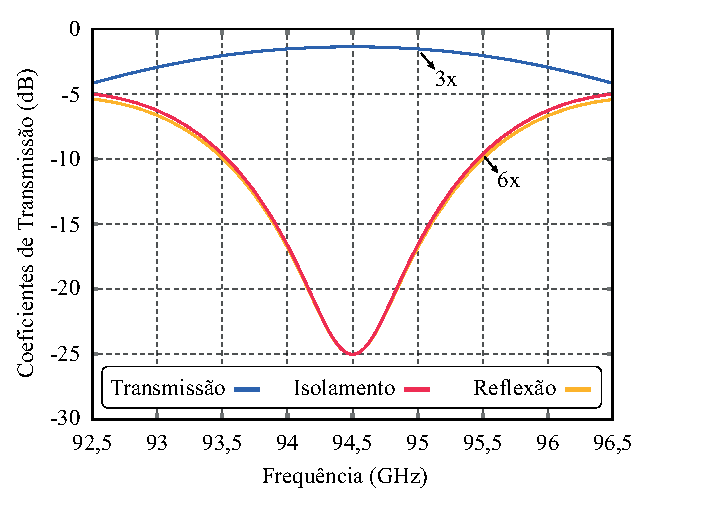
\includegraphics{04-Figuras/PhcTargetFrequencyResponse.eps}
	\caption{Resposta em frequência desejada.} \par
    Fonte: do Autor.
	\label{fig: PhcTargetFrequencyResponse}
\end{figure}

Ambos dispositivos foram projetados para operar na frequência central de 94,5 GHz, portanto, todas as curvas estão em ressonância a essa frequência. As curvas relacionadas ao \textit{isolamento} e a \textit{reflexão} têm os seus coeficientes de transmissão com vale em -25 dB.

É válido ressaltar que essas características de operação idealizadas na Fig. \ref{fig: PhcTargetFrequencyResponse} foram definidas às proximidades de resposta em frequência de simulações já observadas dos referidos dispositivos. Construir uma resposta em frequência desejada muito distante do que o dispositivo habitualmente se comporta, pode levar o modelo em redes neurais a nunca chegar em uma solução. Seria o caso, por exemplo, se as curvas de isolamento e reflexão estivessem com o vale a -200 dB. Certamente, essa poderia ser uma solução intangível no \textit{espaço de design}.
